\section{Cameras and Windows}
\label{chapter:design:windows}

	%\cite{Kolb:1995:RCM:218380.218463} provides a very good introduction to the advanced usage of cameras in virtual environments. 

	We will implement a simplified model of cameras, defined by near- and far clip distances, as well as a field of vision. The aspect ratio will always match that of the render window, preventing accidental distortion of the render output.

	A window is a 2d-plane where the view of a camera can be projected to. As the window is partially managed by the system's window manager and modified by the user of an application, this entity should additionally be regarded as a communication device. The user can move, re-size or close the window. We will only model a single such interaction to prove that the architecture could support others as well. Window objects in our library will be able to detect when the user has closed a window.
	
	\begin{figure}[htbp]
		\centering
		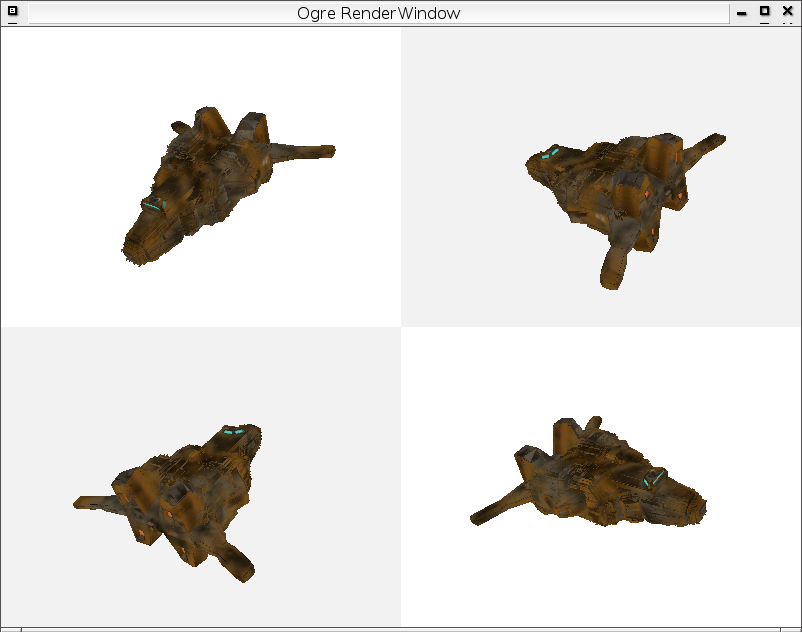
\includegraphics[width=8cm]{images/viewports/viewports.png}
		\caption{A render window displaying a single space ship in four different viewports.}
		\label{fig:ViewportExample}
	\end{figure}

	All our reference engines allow us to partition the render plane of the windows to create multiple smaller regions that each display the rendered output of one camera, as demonstrated by Figure \ref{fig:ViewportExample}. This approach allows developers to implement split-screen games, for example. All three engines provide this feature, although they all use different names for this fraction of the window displaying the output of a camera:

	\begin{smalllist}
		\item Ogre3d calls them \emph{Viewports},
		\item in Panda3d, these are \emph{DisplayRegions}, whereas
		\item OpenScenegraph refers to them as \emph{Views}.
	\end{smalllist}
	
	We will be using the term \classname{Viewport}, as this is the technical term for this construct and the other names do not provide any additional insight into this entity. Figure \ref{fig:WindowCameraAssociation} shows the general association between windows, viewports and cameras\footnote{A viewport is actually not limited to a single camera in all reference implementations, but we will stick to this simple model for our library.}. A viewport contains information on how the camera view is embedded into a window.

	\begin{figure}[htbp]
		\centering
		
\includegraphics[width=8cm]{images/OgreWindowViewport.png}
		\caption{Associations between windows, viewports and cameras.}
		\label{fig:WindowCameraAssociation}
	\end{figure}

	One important property a viewport needs is its \emph{z-index}. This value is consulted whenever viewports overlap. The one with the lower value is drawn first and is overlapped by the viewports ``above'' it.

	The implementation of these structures are described during the implementation of the \classname{Renderer} in Section \ref{chapter:implementation:renderer}.

